\documentclass{beamer}
\usefonttheme[onlymath]{serif}

\mode<presentation> {
	\usetheme{Madrid}}
\usepackage{graphicx}
\usepackage{ucs}
\usepackage[utf8x]{inputenc}
\usepackage[T1]{fontenc}
\usepackage[ngerman]{babel}
\usepackage[ngerman]{varioref}
\usepackage{amsmath,amssymb,amstext,amsthm}
\usepackage{babelbib}
\usepackage[linesnumbered]{algorithm2e}

\newcommand{\R}{\mathbb{R}}
\newcommand{\N}{\mathbb{N}}
\newcommand{\Q}{\mathbb{Q}}
\newcommand{\Z}{\mathbb{Z}}
\newcommand{\Prim}{\mathbb{P}}
%\newcommand{\cha}{\text{$\unlhd$\raisebox{0pt}{$\stackrel{{}_\vert}{}$} }}
%\newcommand{\AutG}{\text{Aut($G$)}}
%\newcommand{\SocHi}{\text{\rm Soc($H_i$)}}
%\newcommand{\bigslant}[2]{\left.\raisebox{.2em}{$#1$}\middle/\raisebox{-.2em}{$#2$}\right.}

%\newcounter{saveenumi}
%\newcommand{\seti}{\setcounter{saveenumi}{\value{enumi}}}
%\newcommand{\conti}{\setcounter{enumi}{\value{saveenumi}}}


\title[Projekt 2]{Fiber-To-The-x}

\author{Lucia Ortjohann und Moritz Hefner}

\institute[]{Netzwerkoptimierung in der Praxis}

\date{16. November 2018}

\begin{document}
	\begin{frame} %C
		\titlepage
	\end{frame}
	
	\begin{frame}{Vor\"uberlegung}
	\begin{itemize}
		\item Jeder Kunde \(k \in K\) hat  eine Nachfrage an Bandbreite von $d(k)$.
		\item Glasfaserkabel liefern unendlich Bandbreite.
		\item Kupferkabel haben eine beschr\"ankte Kapazit\"at, also die Kanten aus $A_2$.
		\vspace{0.8cm}
		\pause
		\item F\"ur alle Kanten aus $ij \in A_2$ \"uberpr\"ufen wir:\\
		Falls die Kapazit\"at der Kante $ij$ kleiner ist als der Bedarf  $d(j)$,
		l\"oschen wir die Kante aus dem Graphen.
		\item Alle Probleme l\"osen wir auf diesem neuen Graphen. 
	\end{itemize}
		
	\end{frame}
	\begin{frame}{Point-to-point mit Glasfaser}
	\scalebox{1}{	\begin{algorithm}[H]
			\label{algP2PG}
			\SetKwInOut{Input}{Eingabe}\SetKwInOut{Output}{Ausgabe}
			\Input{$G=(V,A,c)$}
			\Output{Leitstelle, Netzwerk, Kosten}
			\BlankLine
			
			\ForAll{$l\in L$}{
				\ForAll{$f \in F_1$}{
					Berechne $W_{l,f}$ und $c_{\text{dij}}(\{l,f\})$ mit dem Dijkstra-Algorithmus auf $H=(\{l\} \cup S \cup F , I,c\mid_I)$}
				$C_l:=c(l) + \displaystyle\sum_{f \in F_1} c_{\text{dij}}(lf) + c(f)$. 
			}
			Leitstelle$:=i:=\arg \displaystyle\min_{l \in L} C_l$\\
			Netzwerk$:=(\bigsqcup_{f \in F_1 }W_{i,f}) \cup A_2 $. \\
			Kosten$:=C_{i}$
			\BlankLine
			\caption{Algorithmus zum Lösen des P2PG Problems}
	\end{algorithm}}
	\end{frame}
	
	\begin{frame}{Ergebnisse: P2P mit Glasfaser}
	\begin{table}[h]
		\centering
		\begin{tabular}{c|c|c|c}
			Instanz & Naunyn & Berlin & Vehlefanz \\	
			\hline
			Kosten & 480.722 & 1.388.562 & 7.791.258 \\
			Laufzeit auf PC2 & 0,001s & 0,26s & 2,35s\\
		\end{tabular}
	\end{table} 
	\begin{figure}
		\centering
		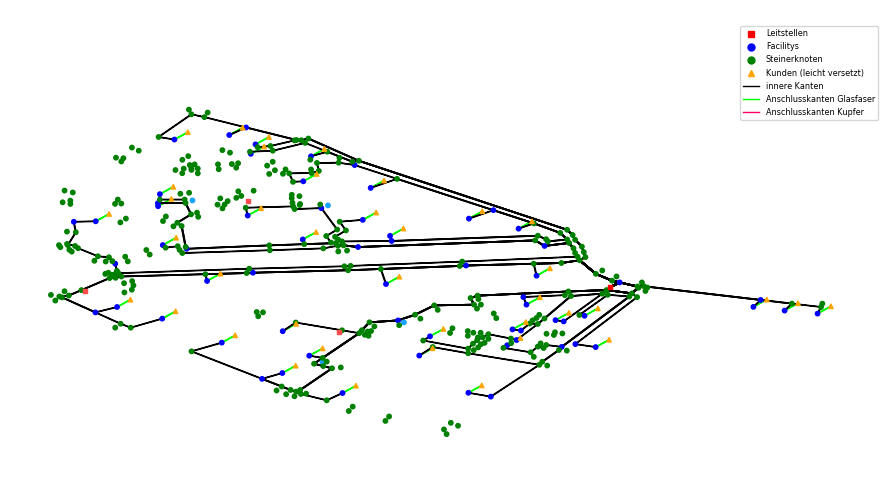
\includegraphics[height=5cm, width=9cm]{./Bilder/P2PG_Berlin} 
		\caption{Berlin}
	\end{figure}
	\end{frame}
	
	\begin{frame}{Ergebnisse: P2P mit Glasfaser und Kupfer}
\begin{table}[h]
	\centering
	\begin{tabular}{c|c|c|c}
		Instanz & Naunyn & Berlin & Vehlefanz \\	
		\hline
		Kosten & 397.662 & 524.392 & 647.608 \\
		Laufzeit auf PC2 & 0,03s & 2,89s & 144,61s \\
	\end{tabular}
\end{table}
	\begin{figure}
			\centering
			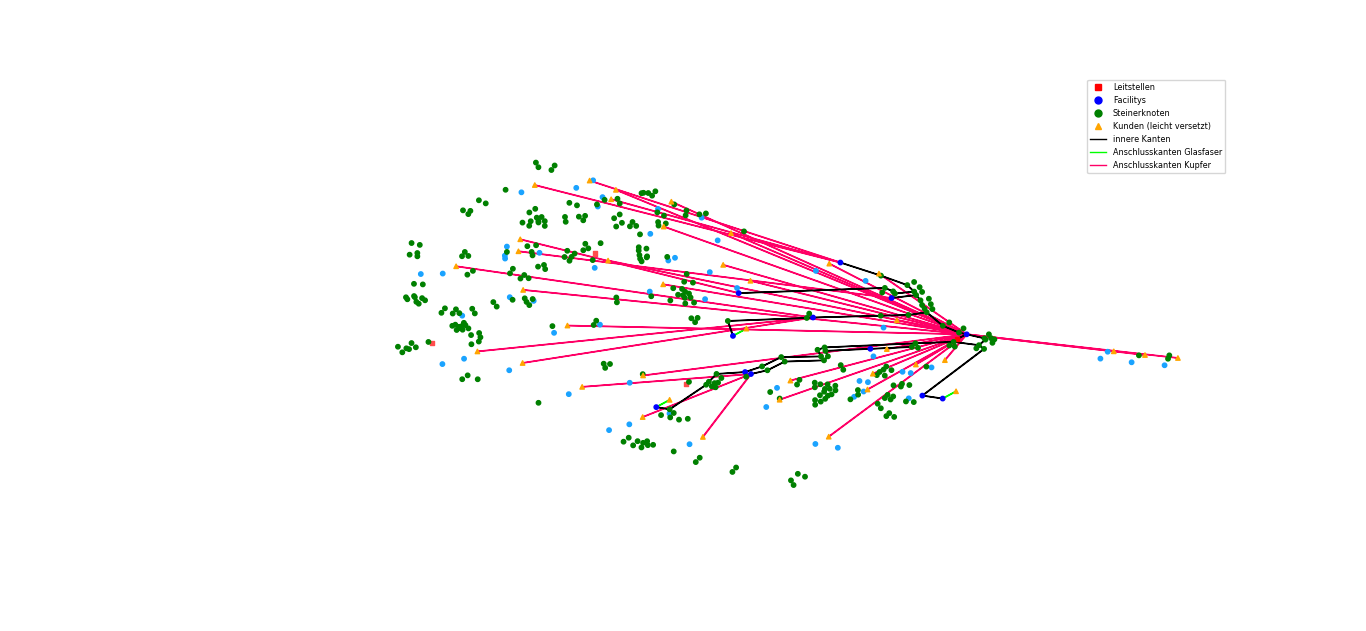
\includegraphics[height=5cm, width=9cm]{./Bilder/P2PGK_Berlin_demand1_duration0} 
			\caption{Berlin}
			\end{figure}
		\end{frame}
	
	\begin{frame}{Point-to-point mit Glasfaser und Kupfer}
\scalebox{1}{	\begin{algorithm}[H]
		\label{alg1}
		\SetKwInOut{Input}{Eingabe}\SetKwInOut{Output}{Ausgabe}
		\Input{$G=(V,A,c)$}
		\Output{Leitstelle, Netzwerk, Kosten}
		\BlankLine
		
		\ForAll{$l\in L$}{
			\ForAll{$f \in F$}{
				Berechne $W_{l,f}$ und $c_{\text{dij}}(\{l,f\})$ mit dem Dijkstra-Algorithmus auf $H=(\{l\} \cup S \cup F , I,c\mid_I)$ mit Startknoten $l$}
			Berechne Steinerbaum $T_l$ auf $H'=(V',A')$ mit Wurzel $l$,\\ Terminals $K \cup \{l\}$ und Kosten $c'$\\
			$C_l:=c(l)+c'(T_l)$ \\
		}
		Leitstelle$:=i:=\arg \displaystyle\min_{l \in L} C_l$\\
		Netzwerk$:=(\bigsqcup_{if \in T_i \cap D}W_{i,f}) \cup (T_i\cap A)$\\
		Kosten$:=C_{i}$
		\BlankLine
		\caption{Algorithmus zum Lösen des P2PGK Problems}
	\end{algorithm}}
	\end{frame}
	
	\begin{frame}{Erweiterung des P2PGK mit Bedarf}
		\begin{itemize}
			\item F\"ur alle Kanten aus $ij \in A_2$ \"uberpr\"ufen wir:\\
			Falls die Kapazit\"at der Kante $ij$ kleiner ist als der Bedarf  $f \cdot d(j)$,
			l\"oschen wir die Kante aus dem Graphen.
		\end{itemize}
\begin{figure}[h]
	\centering
		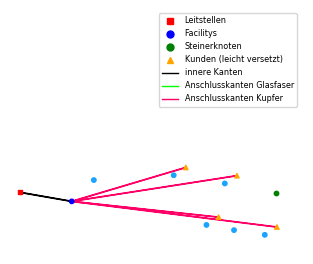
\includegraphics[height=4cm, width=6cm]{./Bilder/P2PGK_Naunyn_demand1_duration0}
	\caption{Lösung des P2PGK mit verschiedenen Bedarfsfaktoren $f = 1$ auf der Instanz Naunyn}
\end{figure}
	\end{frame}
	
		\begin{frame}{Erweiterung des P2PGK mit Bedarf}
			\begin{itemize}
				\item F\"ur alle Kanten aus $ij \in A_2$ \"uberpr\"ufen wir:\\
				Falls die Kapazit\"at der Kante $ij$ kleiner ist als der Bedarf  $f \cdot d(j)$,
				l\"oschen wir die Kante aus dem Graphen.
			\end{itemize}
			\begin{figure}[h]
				\centering
				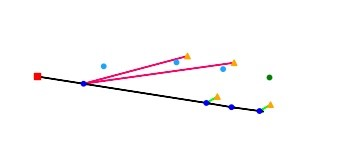
\includegraphics[height=4cm, width=6cm]{./Bilder/P2PGK_Naunyn_demand1_5_duration0_2}
				\caption{Lösung des P2PGK mit verschiedenen Bedarfsfaktoren $f = 1,5$ auf der Instanz Naunyn}
			\end{figure}
		\end{frame}
		
		\begin{frame}{Erweiterung des P2PGK mit Bedarf}
			\begin{itemize}
				\item F\"ur alle Kanten aus $ij \in A_2$ \"uberpr\"ufen wir:\\
				Falls die Kapazit\"at der Kante $ij$ kleiner ist als der Bedarf  $f \cdot d(j)$,
				l\"oschen wir die Kante aus dem Graphen.
			\end{itemize}
			\begin{figure}[h]
				\centering
				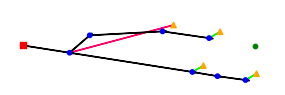
\includegraphics[height=4cm, width=6cm]{./Bilder/P2PGK_Naunyn_demand3_5_duration0}
				\caption{Lösung des P2PGK mit verschiedenen Bedarfsfaktoren $f = 3$ auf der Instanz Naunyn}
			\end{figure}
		\end{frame}

		\begin{frame}{Erweiterung des P2PGK mit Bedarf}
			\begin{itemize}
				\item F\"ur alle Kanten aus $ij \in A_2$ \"uberpr\"ufen wir:\\
				Falls die Kapazit\"at der Kante $ij$ kleiner ist als der Bedarf  $f \cdot d(j)$,
				l\"oschen wir die Kante aus dem Graphen.
			\end{itemize}
			\begin{figure}[h]
				\centering
				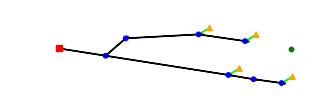
\includegraphics[height=4cm, width=6cm]{./Bilder/P2PGK_Naunyn_demand6_5_duration0}
				\caption{Lösung des P2PGK mit verschiedenen Bedarfsfaktoren $f = 6,5$ auf der Instanz Naunyn}
			\end{figure}
		\end{frame}
		
		\begin{frame}{Erweiterung des P2PGK mit Profit}
			\begin{itemize}
				\item ändere Kostenfunktion
			\end{itemize}
			\begin{align*}
			c': A' \rightarrow \Q, ij \mapsto \left\{\begin{array}{cl} 
			c_{\text{dij}}(lf), & \text{falls } ij \in E \text{ und } j \in F_1\\ 
			c_{\text{dij}}(lf)+c(j), & \text{falls } ij \in E \text{ und } j \in F_2\\ 
			c(ij) + c(i) - t \cdot p_1(j), & \text{falls } ij \in A_1\\ 
			c(ij) - t \cdot p_2(j), & \text{falls } ij \in A_2\\ 
			\end{array}
			\right.
			\end{align*}
			\begin{itemize}
				\item erweitere Steinerbaum Model:
			\end{itemize}
			\begin{align*}
			x_{ij} \leq \displaystyle\sum_{t \in K} y_{ij}^t \quad \forall ij \in A \text{ mit } c(ij) \leq 0
			\end{align*}
			\end{frame}
		\begin{frame}{Erweiterung des P2PGK mit Profit}
			\begin{itemize}
				\item $A_k$ die Anzahl der Kunden mit einem Glasfaseranschluss
			\end{itemize}

			\begin{table}[h]
				\centering
				\begin{tabular}{c|c|c}
					\centering
					Jahre & Kosten & $A_k$ \\	
					\hline
					$0$   	 &  524.392 & 3  \\
					$10$ 	&   366.112& 3  \\
					$20$   	&   207.832 & 3  \\
					$30$    &   49.552 & 3  \\
					$40$    & $-111.448$ & 4 \\
				\end{tabular}
				\label{P2PGKProfit}
				\caption{Ergebnisse des P2PGK mit Profit f\"ur Berlin} 
			\end{table}
		\end{frame}
		
		
	\begin{frame}{Point-to-multipoint mit Glasfaser}
	F\"ur jede Leistelle $l \in L$ l\"osen wir das Model: \\
	\vspace{0.2cm}
	\textbf{Graph:}  $G=(V:=\{l\}\cup S \cup F \cup K ,\: \:   A:= I\backslash I_L \cup A_1$)\\
	\vspace{0.2cm}
	\textbf{Entscheidungsvariablen:}\\
	\begin{tabular}{lll}
			$y_{ij}^t \in \{0,1\}$ &$\forall ij \in A, t\in K $ & modelliert einen Fluss für jeden Kunden $t$ \\
			&&von der Leitstelle $l$ zum Kunden $t$\\
			$x_{ij} \in \Z_{\geq 0}$ & $\forall ij \in A$ &gibt an, wie häufig die Kante in dem \\
			&&Lösungsnetzwerk gekauft wird\\
			$s_i \in \{0,1\}$ & $\forall i \in F \cup S$ & gibt an, ob ein Splitter im Knoten \\
			&&$i\in S \cup F$ gekauft wird ($s_i=1$)\\
			 &&oder nicht ($s_i=0$)
	\end{tabular}

\end{frame}
	
	\begin{frame}{P2MP mit Glasfaser}
	 $\min \displaystyle\sum_{ij \in A} c'(ij) x_{ij} + \displaystyle\sum_{i \in F \cup S} c_s s_i $
	\begin{align*}
\begin{array}{rcrcrcl}
\textrm{s.t.}  
&& &\displaystyle\sum_{ji \in A} y_{ji}^t - \displaystyle\sum_{ij \in A} y_{ij}^t& = & \left\{\begin{array}{cl} 
-1, & \text{falls } i=l\\ 
1, & \text{falls } i=t\\ 
0, & \text{sonst.}\\ 
\end{array}
\right. & \forall t \in K\\
&&& y_{ij}^t & \leq & x_{ij} & \forall ij \in A, t\in K \\
&&& s_i &\leq& \displaystyle\sum_{ji \in A} x_{ji}& \forall  i \in S \cup F\\ 
&0&\geq&\displaystyle\sum_{ji \in A} x_{ji} - \displaystyle\sum_{ij \in A} x_{ij}&\geq& -(a-1)s_i & \forall i \in S \cup F\\
&&& y_{ij}^t & \in & \{0,1 \}& \forall ij \in A, t \in K \\
&&& x_{ij} & \in & \Z_{\geq 0} & \forall ij \in A\\
&&& s_i & \in & \{ 0,1 \} & \forall i \in F \cup S \\
\end{array}
\end{align*}
\end{frame}

\begin{frame}{Ergebnisse: P2MP mit Glasfaser}
\end{frame}

\begin{frame}{Point-to-multipoint mit Glasfaser und Kupfer}
	F\"ur jede Leistelle $l \in L$ l\"osen wir das Model: \\
	\vspace{0.2cm}
	\textbf{Graph:}  $G=(V:=\{l\}\cup S \cup F \cup K ,\: \:   A:= I\backslash I_L \cup A$)\\
	\vspace{0.2cm}
	\textbf{Entscheidungsvariablen:}\\
	\begin{tabular}{lll}
		$y_{ij}^t \in \{0,1\}$ &$\forall ij \in A, t\in K $ & modelliert einen Fluss für jeden Kunden $t$ \\
		&&von der Leitstelle $l$ zum Kunden $t$\\
		$x_{ij} \in \Z_{\geq 0}$ & $\forall ij \in A$ &gibt an, wie häufig die Kante in dem \\
		&&Lösungsnetzwerk gekauft wird\\
		$s_i \in \{0,1\}$ & $\forall i \in F \cup S$ & gibt an, ob ein Splitter im Knoten \\
		&&$i\in S \cup F$ gekauft wird ($s_i=1$)\\
		&&oder nicht ($s_i=0$)\\
		$m_i \in \{0,1\}$ & $\forall i \in F_2$ & gibt an, ob ein Multiplexer in $i\in F_2$\\
		&& installiert wird ($m_i=1$) \\
		&&oder nicht ($m_i=0$)
	\end{tabular}
\end{frame}

\begin{frame}{Point-to-multipoint mit Glasfaser und Kupfer}
	  $\min \displaystyle\sum_{ij \in A} c'(ij) x_{ij} + \displaystyle\sum_{i \in F \cup S} c_s s_i + \displaystyle\sum_{i \in F_2} c(i) m_i$
	  \begin{align*}
	  \begin{array}{ccrcl}
	  \textrm{s.t.}  
	   &\displaystyle\sum_{ji \in A} y_{ji}^t - \displaystyle\sum_{ij \in A} y_{ij}^t& = & \left\{\begin{array}{cl} 
	  -1, & \text{f. } i=r\\ 
	  1, & \text{f. } i=t\\ 
	  0, & \text{sonst.}\\ 
	  \end{array}
	  \right. & \forall t \in K \\
	  & y_{ij}^t & \leq & x_{ij} & \forall ij \in A, t\in K \\
	  & s_i &\leq& \displaystyle\sum_{ji \in A} x_{ji}& \forall  i \in F \cup S \\ 
	  0\geq&\displaystyle\sum_{ji \in A} x_{ji} - \displaystyle\sum_{ij \in A} x_{ij}&\geq& -(a-1)s_i & \forall i \in S \cup F_1\\
	  0\geq&\displaystyle\sum_{ji \in A} x_{ji} -m_i - \displaystyle\sum_{ij \in I \cup A_1} x_{ij}&\geq& -(a-1)s_i & \forall i \in F_2\\
	  &s_i+m_i & \leq & 1 & \forall i \in F_2 \\
	  &x_{ij}& \leq & m_i & \forall i \in F_2 \\
	  \end{array}
	  \end{align*}
\end{frame}

\begin{frame}{Ergebnisse: P2MP mit Glasfaser und Kupfer}
\end{frame}
	
\begin{frame}{Erweiterung des P2MPGK mit Bedarfserhöhung}

\end{frame}

\begin{frame}{Erweiterung des P2MPGK mit Profit}
	
\end{frame}

\begin{frame}{Zusammenfassung}

\end{frame}

	
\end{document}